	\section{Domain} 
		\subsection{Domainmodel}
	
		\subsection{Verknüpfungen von Task-Vorlagen und Entscheidungs-Vorlagen}
			Wissensproduzenten können Task-Vorlagen an Entscheidungs-Vorlagen zuordnen.
			Dabei kann und soll auch eine Task-Vorlage an verschiedene Entscheidungs-Vorlagen zugeordnet werden.
			Ebenso können Entscheidungs-Vorlagen natürlich mehrere Task-Vorlagen zugeordnet erhalten.
			
			\subsubsection{Arten der Zuordnung}
				Task-Vorlagen können mit Entscheidungs-Vorlagen auf zwei Arten verknüpft werden.
				Sie können entweder dann fällig werden, wenn eine Entscheidung getroffen wurde (operativer Task).
				Oder eine Task-Vorlage ist da um eine Entscheidung zu treffen (Entscheidungstask).
				Auf die Task-Vorlagen selbst hat dies jedoch keinen Einfluss, sie sind unabhängig davon.

			\subsubsection{Übertragung in \ppt}
				Aus diesen Task-Vorlagen werden beim Übertag in ein \ppt\ Tasks generiert.
				Task-Vorlagen sind generisch, da Änderungen auch alle verknüpften Entscheidungs-Vorlagen betreffen sollen.
				Aus diesem Grund werden Task-Vorlagen bei der Zuordnung verknüpft und nicht kopiert.
				
				\begin{figure}[H]
					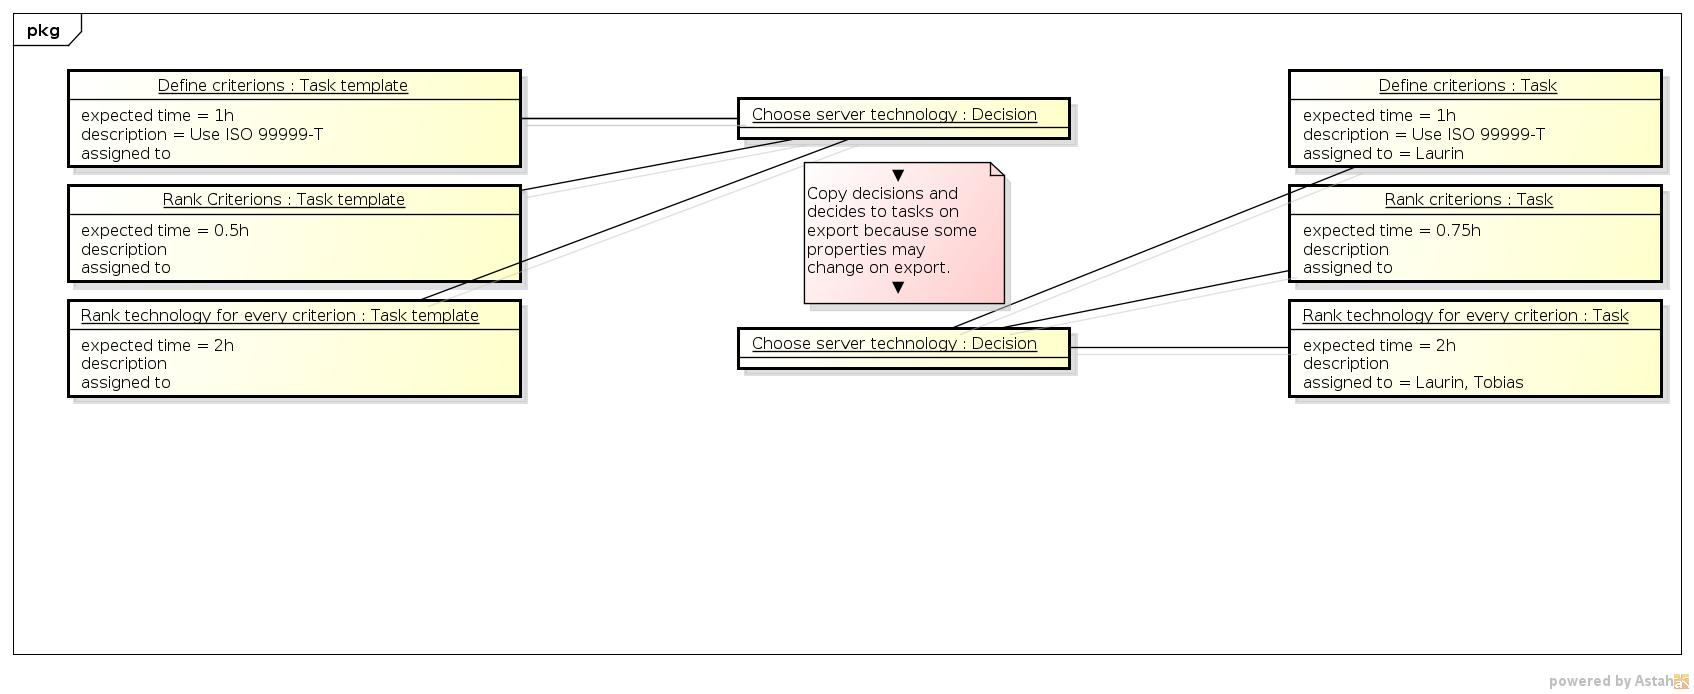
\includegraphics[width=\textwidth]{architecture/media/img/DecisionTaskRelation.jpg}
					\centering
					\caption{Exportieren von Entscheidungen}
					\label{fig:DecisionTaskRelation}
				\end{figure}
				
				Beim Exporten werden aus Task-Vorlagen (konkrete) Tasks.
				Auch Entscheidungen werden zu Tasks.
				Mit Entscheidungen verknüpfte Tasks werden dann zu Sub-Tasks.
				
				Benutzer wollen beim Export die von der Task-Vorlage vorgegebenen Werte möglicherweise anpassen, wie z.B. den erwarteten Aufwand für den Task.
				Daher ist es sinnvoll, die Eigenschaften der Task-Vorlagen in die (konkreten) Tasks zu kopieren, anstatt sie lediglich zu verknüpfen.
				Gleiches gilt für Entscheidungen. Würde jemand im CDAR diese verändern oder Löschen, so würde dies die History zerstören.
			
		
		\subsection{EEPPI Domain}
			
				
		
		\subsection{Communication}